
\documentclass[11pt]{article}
\usepackage{tabto}
\usepackage{hyperref}
\usepackage{graphicx}
\usepackage{float}
\begin{document}


\begin{titlepage} 
	\newcommand{\HRule}{\rule{\linewidth}{0.5mm}} 
	
	\center 
	
	\textsc{\LARGE CS 130: Software Engineering}\\[1.5cm] 
	
	\textsc{\Large Professor: Miryung Kim}\\[0.5cm] 
	
	\textsc{\large TA: Brett Chalabian}\\[0.5cm] 
	

	
	\HRule\\[0.4cm]
	
	{\huge\bfseries Name}\\[0.4cm] % Title of your document
	{\huge\bfseries Part A Report}\\[0.4cm]
	\HRule\\[1.5cm]
	

	
			\large
			\textit{Team Members}\\
			Vishaal Agartha, Kelvin Zhang, Karen Zhang, Albert Pan, Anav Sanghvi, CJ Ordog

	

	
	\vfill\vfill\vfill 
	
	{\large\today} 
	\vfill
	Project URL:  \url{https://github.com/vishaalagartha/CS130-project}

	 
	
	\vfill 
	
\end{titlepage}

\section{Motivation}
\tab With the data-driven and opinion overload information era on the rise, it is imperative for us to efficiently understand and parse the gist of large text documents. These text documents are shifting towards opinionated articles from Facebook posts or bloggers, for example, rather than bland factual regurgitation from a textbook or newspaper. This movement has lead to a relatively new field of Computer Science termed sentiment analysis or the process of computationally classifying an opinionated piece of text as positive, negative, or neutral.
Sentiment analysis can be conducted via manual processing, keyword processing, or natural language processing. Obviously, manually processing is not viable for a large document and keyword processing is often inaccurate and too simple to capture the complexity of languages. Hence, we suggest using machine learning in conjunction with natural language processing to accurately categorize opinionated text.
\\
\par This approach has been adopted and used for various platforms, including Twitter, Facebook, and several newspapers. However, it has not been implemented in a user-friendly manner for a niche community of the web - Reddit. We believe Reddit is an excellent candidate for sentiment analysis because it drills into a community of interested candidates and captures a wide variety of opinions. By performing sentiment analysis on a specific subreddit, we can get the general idea of how engaged experts in a certain field feel about a certain subject.
\section{Feature Description and Requirements}
\tab We plan on providing a simple user interface, where any user can specify a specific subreddit or community and a date range. Based on the parameters, the data collected by the web scraper will be sent to a backend server for data analysis. To make our application more interactive and user-friendly on the front end, we also plan on visualizing the data in a world cloud. A word cloud is an image composed of words in an appealing manner where the size of the word is proportional to its relative frequency in the document.

 \begin{figure}[H]
 	\centering
 	 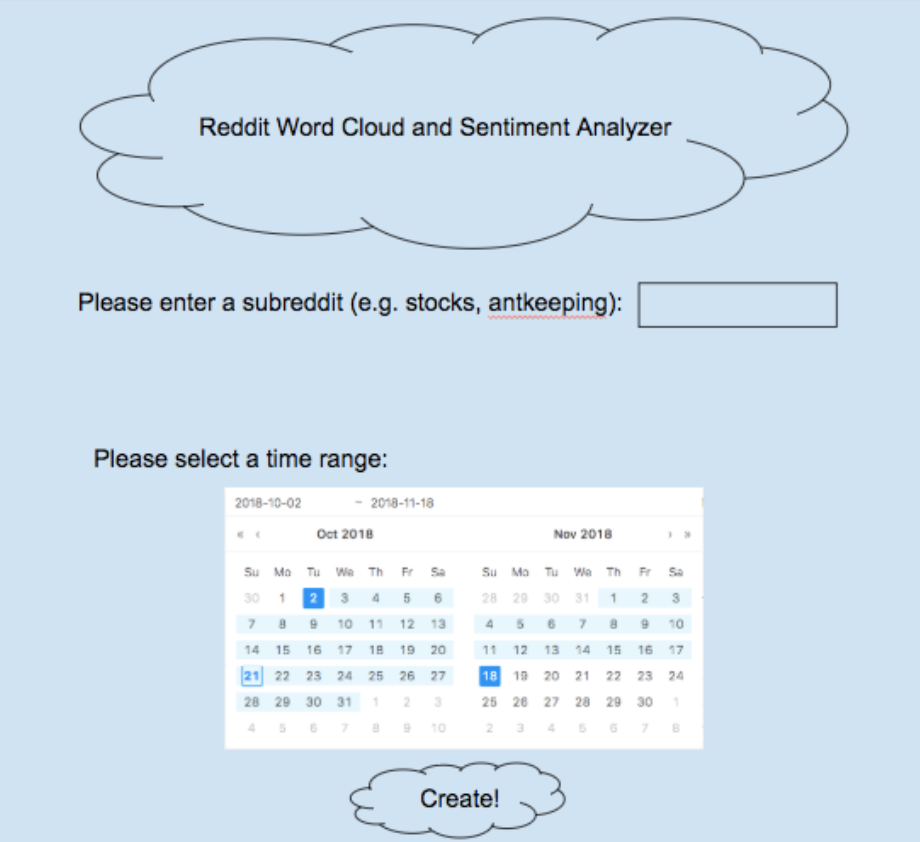
\includegraphics[scale=0.6]{landing}
 	\caption{Landing page where user can specify parameters for the word cloud they wish to 	generate.}
 \end{figure}

\subsection{Backend}
\tab The server will then take these input parameters and parse all relevant headlines, comments, and subcomments from the subreddit and calculate the most frequently appearing words according the input parameter. Obviously, we will ensure that frequently appearing irrelevant words such as ‘the’ or ‘is’ will be filtered out. Next, these relevant words will be fed into our previously trained machine learning algorithm, which will calculate the sentiment towards the relevant word. The server will then return a hashable type containing all the relevant words and the sentiment towards the words. After this processing, we will render the word cloud where frequency is proportional. 

\subsection{Frontend}

 \begin{figure}[H]
 	\centering
 	 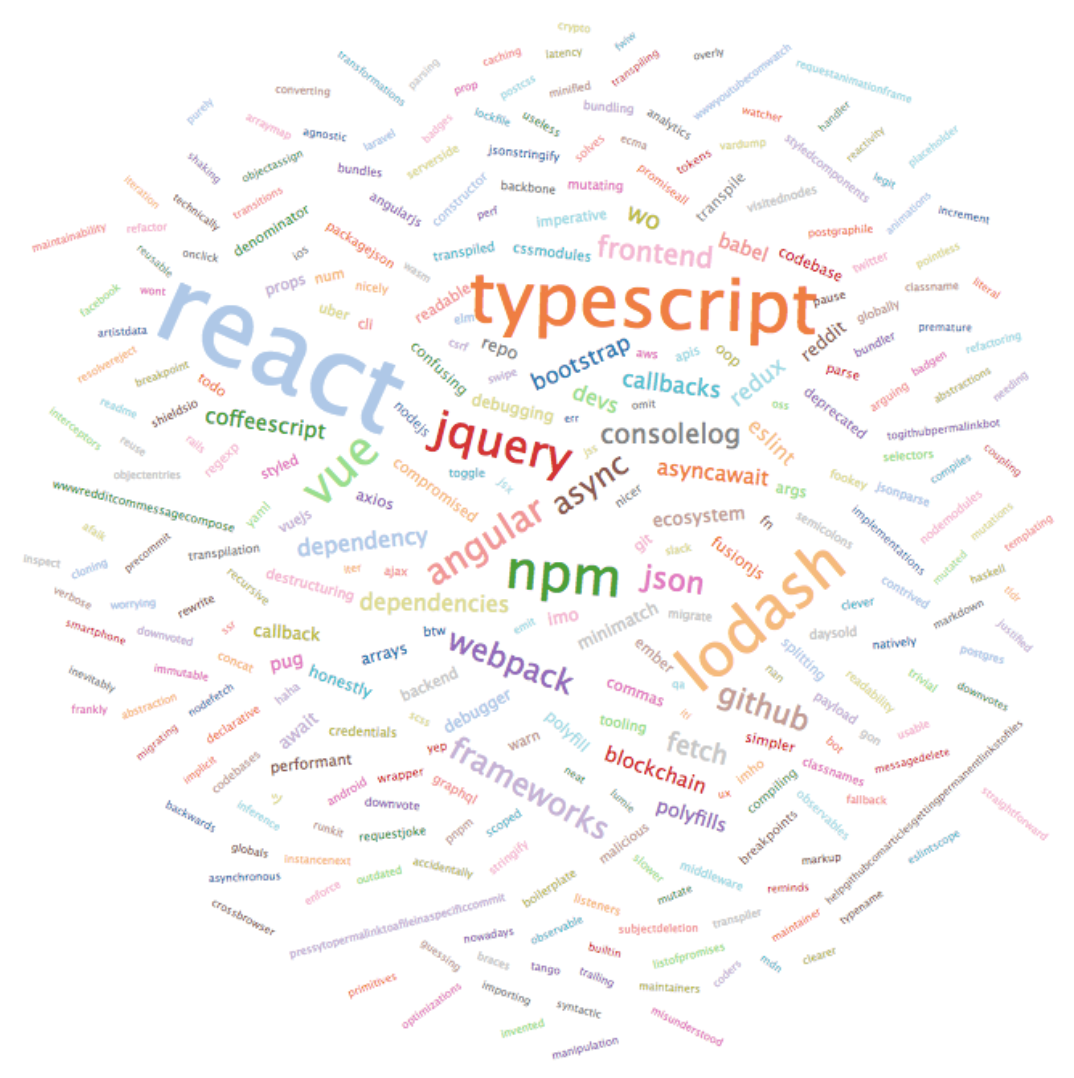
\includegraphics[scale=0.3]{word_cloud}
 	\caption{A sample word cloud that our algorithm will be able to generate.}
 \end{figure}

\tab Moreover, a user will be able to over a certain word, at which point the word will become bold and highlighted. Once the user selects the word, we will include a chart to the right of the word cloud to display the sentiment analysis data.

 \begin{figure}[H]
 	\centering
 	 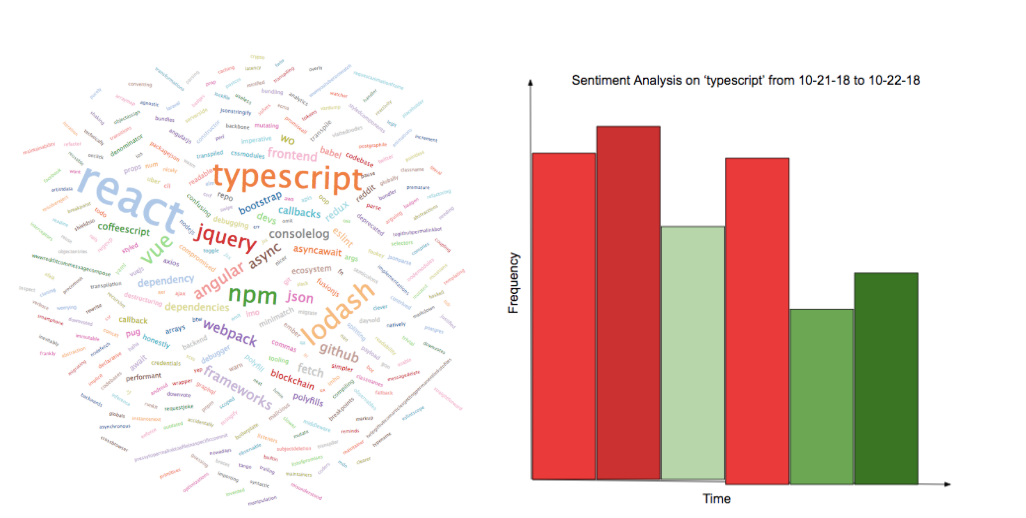
\includegraphics[scale=0.5]{graph}
 	\caption{A sample rendering of the screen once the user has selected ‘typescript’. This creates a bar chart where the x-axis is time within the selected range (10-21-18 to 10-22-18) and the y-axis is the relative frequency. Finally, the color corresponds to the sentiment toward the word. For example, we can see that ‘typescript’ was not very popular at the start of the day, but became more popular as the day went on.}
 \end{figure}

\subsection{Usage}
\tab Despite the application’s simplicity, we cater to multiple users rendering it highly useful. Consider the following usage scenarios:

\begin{enumerate}

\item{Magazine or Newspaper article writer searching for a captivating visualization}

\par Consider a news piece writer trying to capture the sentiment and thoughts of a highly extremist political group. They may consider generating a world cloud via using the subreddit r/The\_Donald, a subreddit dedicated that describes itself as ‘a never-ending rally dedicated to the 45th President of the United States, Donald J. Trump’. From this visualization, we could understand how this community feels about the highly volatile news regarding our President.

\item{Celebrity trying to understand what a certain community feels about them
}

\par Consider a famous athlete or actor who recently made a big decision and wishes to understand how his fans took it. For example, basketball superstar LeBron James decided to switch teams from the Cleveland Cavaliers to the Los Angeles Lakers this summer. He may browse and look at the sentiments on r/lakers and r/clevelandcavs prior to and after making his decision to see where their loyalties lie. Naturally, since he is a big topic, the word cloud would contain his name and he could simply click on his name to see their sentiments over the timespan.

\item{Stock Market investor}

\par Consider a stock market investor trying to decide whether to buy or sell a certain stock. He or she may want to know what other investors and fans of the company feel about the stock right now. This type of analysis would’ve been highly useful for an investor in Tesla directly after the recent Elon Musk Twitter fiasco. An investor would’ve likely been able to browse r/tesla or r/electricvehicles to see whether the stock price would rise or plummet.

\item{Getting reviews on recent product releases}

\par A user trying to make a decision between two new products may want to see the prominent features and obtain feedback on the two different products. Reddit provides a niche community of experts where users can gain an understanding of which features are relevant and popular. For example, an individual trying to decide between buying a FitBit and a Garmin may want to see the prominent features of each piece of technology via word cloud and see the sentiment towards them.
\end{enumerate}

 \begin{figure}[H]
 	\centering
 	 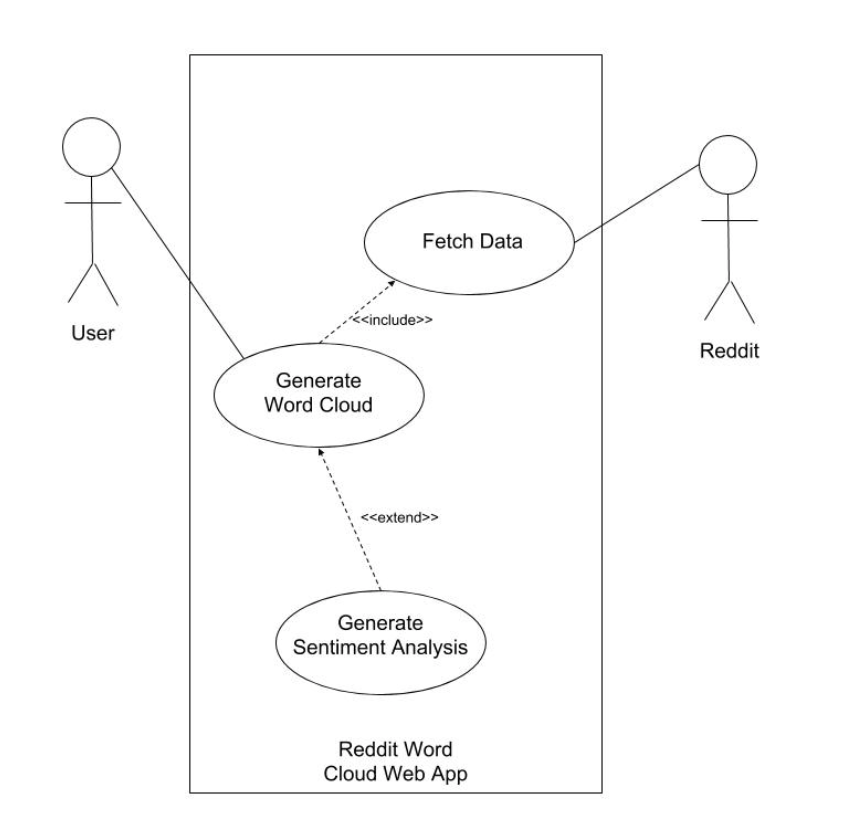
\includegraphics[scale=0.6]{use_case}
 	\caption{Sample use case diagram for the application. Once a user enters a query, the application will fetch data by querying Reddit’s API and generate the word cloud based on frequency. If a user then clicks on a certain word, the application will generate sentiment analysis.}
 \end{figure}
 
\section{Feasibility}
\tab This project is feasible to implement because are familiar with the APIs we plan on using. We are very confident that a standard web application with a responsive front-end will be well completed. We are a little skeptical on how efficient our sentiment analysis and backend will be in terms of performance. In order to scrape and analyze all the comments on a extremely popular thread for a long duration of time, we will need to parallelize the web scraping with Hadoop (Map Reduce). The other efficiency issues we expect to run into is during the logistic regression for sentiment analysis on comments. We are currently debating between using Redis (in-memory data storage/caching) or a traditional SQL database to store previous results and improve time taken to perform sentiment analysis.

\section{Capability}
\tab We have broken down the proposed application into concrete steps and elements. These elements include: front-end design for the user, fetching and filtering data from the subreddit, sentiment analysis, word cloud rendering, and sentiment analysis rendering. These tasks are distributed among our team members as follows:

\subsection{Front-end designer - Kelvin Zhang}
\tab Kelvin has several internships where he worked on full stack web development in both internal and client facing products. He has experience iterating quickly and working in a small team or startup environment. Specific examples of his past work include fully rebuilding the front end of an internal deployment tool in React and addressing stories such product design changes and building APIs. He has also taken relevant courses such as CS143 Databases and 144 Web Applications.

\subsection{Fetching and filtering data - Vishaal Agartha}
\tab Vishaal is a proficient programmer in Python and has worked on multiple applications in the language. His most recent one were for internships at a Blockchain startup known as Unit-E where he used developed a simulator for different proof-of-work and proof-of-stake algorithms to test the algorithm’s transaction throughputs and finalization latencies. Prior to that, Vishaal also worked with a health and fitness based startup known as Simigence where he used unsupervised clustering techniques to learn a user’s ‘primary’ locations. Additionally, he also helped develop a distributed systems tracing infrastructure for logging remote procedure calls.
	\par Vishaal is also an avid Reddit user and frequent participant in rockclimbing, computer science, algorithmic trading, and sports subreddits. He plans on leveraging and has prior experience using the PRAW. PRAW, an acronym for “Python Reddit API Wrapper”, is a way of accessing Reddit’s API via Python.

\subsection{Machine Learning Computation - Albert Pan and Anav Sanghvi}

\tab Albert has experience working on data science and machine learning projects, and has recently completed an internship where he worked on creating a model that would be able to assess the quality of an ad. He has also taken courses on Udemy and Udacity to increase his experience in working with real-world data. Albert has experience working with multiple teams, both small and big.
	\par Anav has experience working on classifying medical images and implementing classifiers for difference kind of diseases. He has also worked on projects to improve performance of data analysis and optimize efficiency of backend via caching/database storage. Anav has also worked on collecting research fields from academic publications to create word clouds to find most frequent topics of research and clusters to find similar research topics for different departments. For this project, he will be working with Albert to create a sentiment analysis model to classify the comments.

\subsection{World Cloud Rendering - CJ Ordog}

\subsection{Sentiment Analysis Chart - Karen Zhang}
\tab At school, Karen Zhang has taken both CS 143 and CS 144, where she learned about databases and web application. She also has previous internship experience where she worked as a full stack developer. For front-end features, she worked closely with React to enhance user experience.

\end{document}
